\section{Theory and experimental setup}
\subsection{Radioactive decay}
Radioactive decay is the process by which an unstable atom transitions to a more stable form through the emission of energy by radiation.
Decay occurs in three main kinds, each associated with a radiation of different nature and properties: $\alpha$-decay, $\beta$-decay and $\gamma$-decay\footnote{Sans le tiret?}.
\begin{itemize}
    %
    \item $\alpha$-decay represents the disintegration of a heavy parent nucleus to a daughter through the emission of a nucleus of helium.
    These particles, accordingly called $\alpha$ particles, are the most energetic between the three forms of radiation (with typical energies of about 5 MeV), but also the least penetrating, being able to be stopped by a sheet of paper.
    %
    \item $\beta$-decay is instead the transformation of a nucleus with an unstable ratio of protons to neutrons into a stabler one by emitting an electron ($\beta^-$ particle), in the case of a proton-rich nucleus, or a positron ($\beta^+$ particle), in the case of an over-abundance of neutrons.
    Additionally, a proton-rich nucleus can also reduce its charge by the absorption of an atomic electron, in a process called \emph{electron capture}.
    The electron comes most often from the inner $K$-shell, resulting in the outer electrons cascading down to fill the lower levels and emitting [one or more] X-rays\cite{intro_nuclear_particle_physics}.
    Of smaller ionising power than $\alpha$ radiation, $\beta$ radiation is however more penetrating, requiring aluminium sheets to be stopped.
    %
    \item $\gamma$-decay, on the other hand, occurs for the most part right after a heavy nucleus desintegrates by emitting an $\alpha$ particle or a $\beta$ particle.
    The daughter nucleus may be left in an excited state and it can deexcite by rearranging the structure of the nuclear shells, 
    a process which is tied to the emission of a high-energy photon (a $\gamma$ ray).
    The typical energies of nuclear $\gamma$ rays range from a fraction to several MeV 
    and though they have the least ionising power of the three, they are the most penetrating, requiring lead for effective shielding.
\end{itemize}

\subsection{Scintillation detectors} \hl{Mettre après? (lire TODO)}
Scintillation detectors are based on the properties of scintillators, materials that emit photons in the visible spectrum after the passage of a charged particle.
The scintillators used for particle detection are primarily [split] between two types: organic (or plastic), in which the photon emission has molecular origin, 
and inorganic (or crystalline), crystals which are doped with activators that can first be excited by electron-hole pairs 
produced by the charged particle passing in the crystal lattice\footnotemark\ and then de-excited by photon emission\cite{intro_nuclear_particle_physics}.
\hl{In this experiment, an inorganic NaI scintillator was used.}

Because of the low intensity of the emitted light, the photon signal must be amplified in order to be properly counted.
This amplification is commonly achieved through the use of photomultiplier tubes (PMT), a device which converts the photon signal in a detectable electric pulse.
It consists of a vacuum chamber containing several components, pictured in Fig. \ref{fig:photomultiplier}: 
after passing a transparent entry window, adjacent to the scintillator, the scintillation photons first encounter a photocatode, 
where they produce an electron by photoelectric effect with a certain probability $\varepsilon$ (the quantum efficacy).
Next, a series of dynodes accellerate the electrons and multiply them through secondary emission.
The anode located at the end of the chamber then allows to read the amplified electric signal, 
which results linearly proportional to the amount of light incident on the photocathode.
The voltage applied between cathode and anode determines the value of the total gain $G$.
\footnotetext{Ici je pourrai écrire "produced by the passing charged particle" sans specifier, pour rendre la phrase un peu plus legere. Or "Excited by th epassing charged particles through [the production of ]electron-hole pairs}
%
\begin{figure}[htbp]
    \centering
    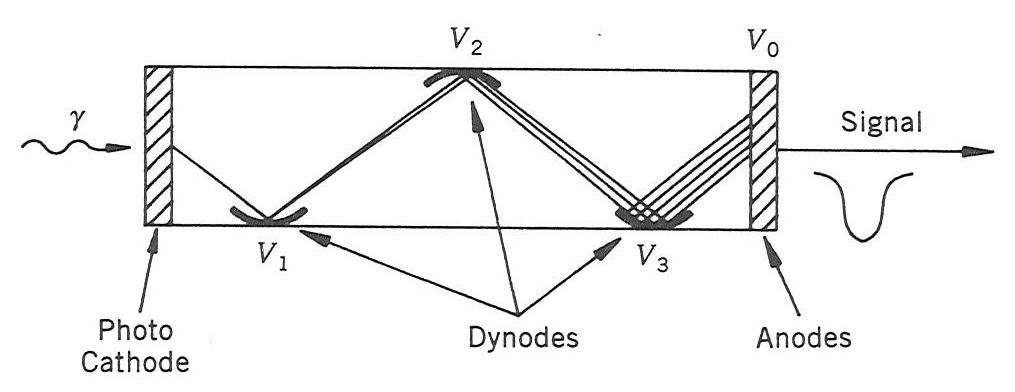
\includegraphics[scale=1.2]{figures/photomultiplier.jpg}
    \caption{Main elements of a photomultiplier tube \cite{intro_nuclear_particle_physics}.}
    \label{fig:photomultiplier}
\end{figure}

[After obtaining the electric signal as output of the PMT], [several electronics elements] allow to obtain the $\gamma$ ray energy spectrum of the studied source, 
showing the intensity of $\gamma$ radiation versus the energy of each photon.
Another amplifier.
A band analyser?? working as discriminator?? allows to select a window of signal amplitudes and create digital signals.
Delay gates can be used to delay \hl{(duh)} the analog signal in order to better match the digital coming from the discriminateur

[The detector, together with the rest of the chaine de spectrometrie] allows to obtain the $\gamma$ ray energy spectrum of the studied source, showing the intensity of $\gamma$ radiation versus the energy of each photon.
The spectrum will not only show [the actual emission], though.
When $\gamma$ rays enter the scintillator, they can interact in two possible ways: through the photoelectric effect or through Compton scattering.
Any photon converted to an electron by photoelectric effect generally deposits its entire energy within the scintillator, such that the intensity of the subsequent scintillation light is proportional to the energy of the original photon.
In the case of Compton scattering, instead, the photons do not deposit all of their energy and, once scattered, can produce new interactions.
A third way would be through $e^+ e^-$ pair production, which is however very unlikely for low-energy photons.

The energy deposited in the crystal will therefore have two kinds of contributions to the $\gamma$ spectrum.
First, the full energies of any of the photons that convert into photoelectrons, and second, a continuous spectrum of energies related to Compton scattering.

There are [some things], though, that will modify the expected appearance of the spectrum.
\begin{itemize}
    \item \hl{Itemize seulement pour mettre en clair, mieux de ne pas prendre trop d'éspace}
    \item The $\gamma$ rays scattered by Compton effect can interact again with the scintillator.
    \item \hl{pic d'échappement? j'ai pas compris pleinement}
    \item Parasite contributions from photons scattered in the material entouring the scintillator, which can be removed with appropriate collimation
    \item The resolution in energy of the scintillator \hl{pas clair}
\end{itemize}

\paragraph{Attenuation in matter}
The [three ways in which photons interact with matter] cause an attenuation of $\gamma$ radiation, i.e. a progressive reduction in the number of photons, without a loss of their individual energy.
This phenomenon follows an exponential law and can be described in terms of a linear attenuation coefficient $\mu$, which depends on the energy of the incident light and the nature of the material.
In fact, let $I(x)$ be the intensity of photons at any point $x$ in the medium.
The change in intensity $dI$ in an infinitesimal thickness of material $dx$ can be written in terms of $\mu$ as follow:
\begin{equation}
    dI = I(x + dx) - I(x) = -\mu(E_{\gamma}, Z) I(x) dx
\end{equation}
where the negative sign indicates that the intensity decreases with travel.
Integrating the previous expression yields the attenuation law
\begin{equation} \label{eq:attenuation_law}
    I(x) = I_0 e^{-\mu(E_{\gamma}, Z) \, x}
\end{equation}
where $I_0$ is the value of the intensity at $x=0$. 
The law can also be put in a different form:
\begin{equation} \label{eq:attenuation_law_density}
    I(x) = I_0 e^{-\mu_d(E_{\gamma}, Z) \, d}
\end{equation}
where, if $\rho$ is the density of the material, $\mu_d = \mu / \rho$ is its mass attenuation coefficient and $d = \rho \cdot x$ its surface density.

\subsubsection{Coincidences}
\begin{figure}[h]
    \centering
    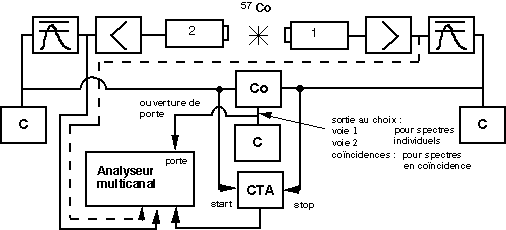
\includegraphics[width=0.75\textwidth]{figures/coincidences.png}
    \caption{Experimental setup for coincidence detection. \cite{notice_VI}}
    \label{fig:setup_coincidences}
\end{figure}

To detect desintegrations that cascade from another excited state, the setup shown in \hbox{Fig. \ref{fig:setup_coincidences}} is used. 
Two scintillators, 1 and 2 are placed on opposite sides of the sample to study\footnote{The studied sample}. 
A coincidence \hl{mettre en emph} occurs whenever an event is measured simultaneously in both detectors. 
\hl{The coincidence module has a time resolution:}
The maximum time resulution \(2 \theta\) is then defined as the maximal time difference between the two impulses from the scintillators.
\begin{equation}
    2 \theta = \theta_1 + \theta_{2}
\end{equation}
Using the counters denoted "C" \hl{emph?} in the diagram, the count rate for impulses outputed from the scintillators 1 and 2, and the coincidence detector are \(m_1\), \(m_2\) and \(m_{12}\). 
\hl{Dire que m1 et m2 viennent des singulars detectors, alors que m12 des deux ensemble au meme temps}

\begin{wrapfigure}{R}{0.5\textwidth}
    % [trim={left bottom right top},clip]
    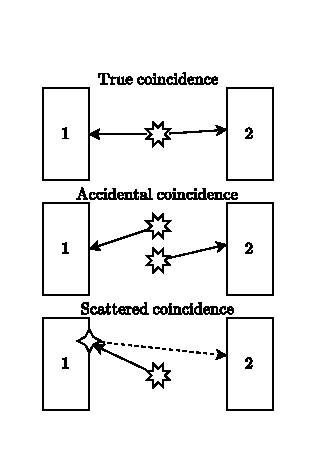
\includegraphics[width=\linewidth, trim={0 1cm 0 1.2cm}, clip]{figures/coincidence_types.pdf}
    \caption{Types of coincidences TODO: MAKE SMALLER, PLACE BETTER}
\end{wrapfigure}
Due to the random nature of radioactivity, there are multiple types of coincidences\footnote{there are multiple ways in which coincidences can be produced}:
\begin{itemize}
    \item True coincidences: the measurement in both detectors\footnote{the detection in both counters} of particles from the same desintegration
    \item Background noise, for example due to cosmic particles \footnote{detailler un peu plus: seulement cosmic particles?}
    \item Accidental: detection of a particle in each detector within the time resolution due to 2 different desintegrations
    \item Scattered: due to Compton scattering, a particle detected in one detector might send a particle back to the second detector.
\end{itemize}

Due to the different types of coincidences, the mesured coincidence rate is
\begin{equation}
    m_{12} = m_t + m_c + m_a
\end{equation}
where \(m_t\) is the true coincidence rate for the studied phenomenon, \(m_c\) is due to the cosmic noise, and \(m_a\) is the accidental coincidence rate. In this experiment, the cosmic noise is assumed to be \(0\) due to the lead shielding used around the detectors and the source. Assuming the outputs of the scintillators correspond to two independent poissonian random variables, the accidental coincidence rate can be linked to the measured rates with
\begin{equation}
    m_a = 2\theta m_1 m_2.
\end{equation}
From this, the true coincidence rate is found to be
\begin{equation}
    m_t = m_{12} - m_c - 2\theta m_1 m_2
\end{equation}

\paragraph{Determining the resolution}
The resolution \(2 \theta\) of the setup can be found by using a source emitting only a single particle per desintegration, such as \cesium. This means that the coincidence rate is purely due to accidental coincidences (\(m_t = 0\)). Thus, the resolution is found to be
\begin{equation}
    2\theta = \frac{m_{12}}{m_1 m_2}.
\end{equation}

\paragraph{Activity of the source}
The measured rates can also be expressed in terms of the activity \(A\) of the source and the probability \(p_1,\ p_2\) of detecting a particle in the scintillator 1, 2:
\begin{equation}
    \begin{aligned}
        m_1 &= A p_1 \\
        m_2 &= A p_2 \\
        m_t &= A p_1 p_2 \\
        m_a &= 2\theta m_1 m_2 = 2\theta A^2 p_1 p_2
    \end{aligned}
\end{equation}
Solving for the activity \(A\) gives
\begin{equation}
    A = \frac{m_1 m_2}{m_t} = \frac{m_1 m_2}{m_{12} - m_c - 2\theta m_1 m_2}
\end{equation}